\chapter{Design \& Implementation}
\label{ch:design}

This chapter will introduce the design and implementation of the project in part. From the overall design of the system, Unified Modeling Language (UML) will be demonstrated next, and the detailed components of the application are indicated in the following with the order from data collection and preprocessing, UI design, to the back-end algorithms.

\section{Overall Design}

To meet the objectives of the project, the graphical architecture of the system is demonstrated in the following Figure \ref{fig:14}. The general design is divided into two parts, front-end operations and back-end algorithms. According to Figure \ref{fig:14},  the rectangles refer to the main processes of the project, and the parallelograms denote the input data or output products of the steps.


The left side of the diagram indicates the front-end operations, containing two simple processes: uploading data and receiving the visualisation result. While the right side illustrates the back-end processes, and the main steps are: 1) collecting the training data including resume dataset and job description dataset, 2) parsing and preprocessing the data, 3) analysing and understanding the features of data by word count, POS distribution, etc., 4) designing and training the models for different aims such as information recognition, skill extraction, etc., 5) applying the models on the input data from user to get the general feedback of the resume and the matching result between the uploaded resume and job description.

\label{overall_design}

 \begin{figure}[H]
    \centering
    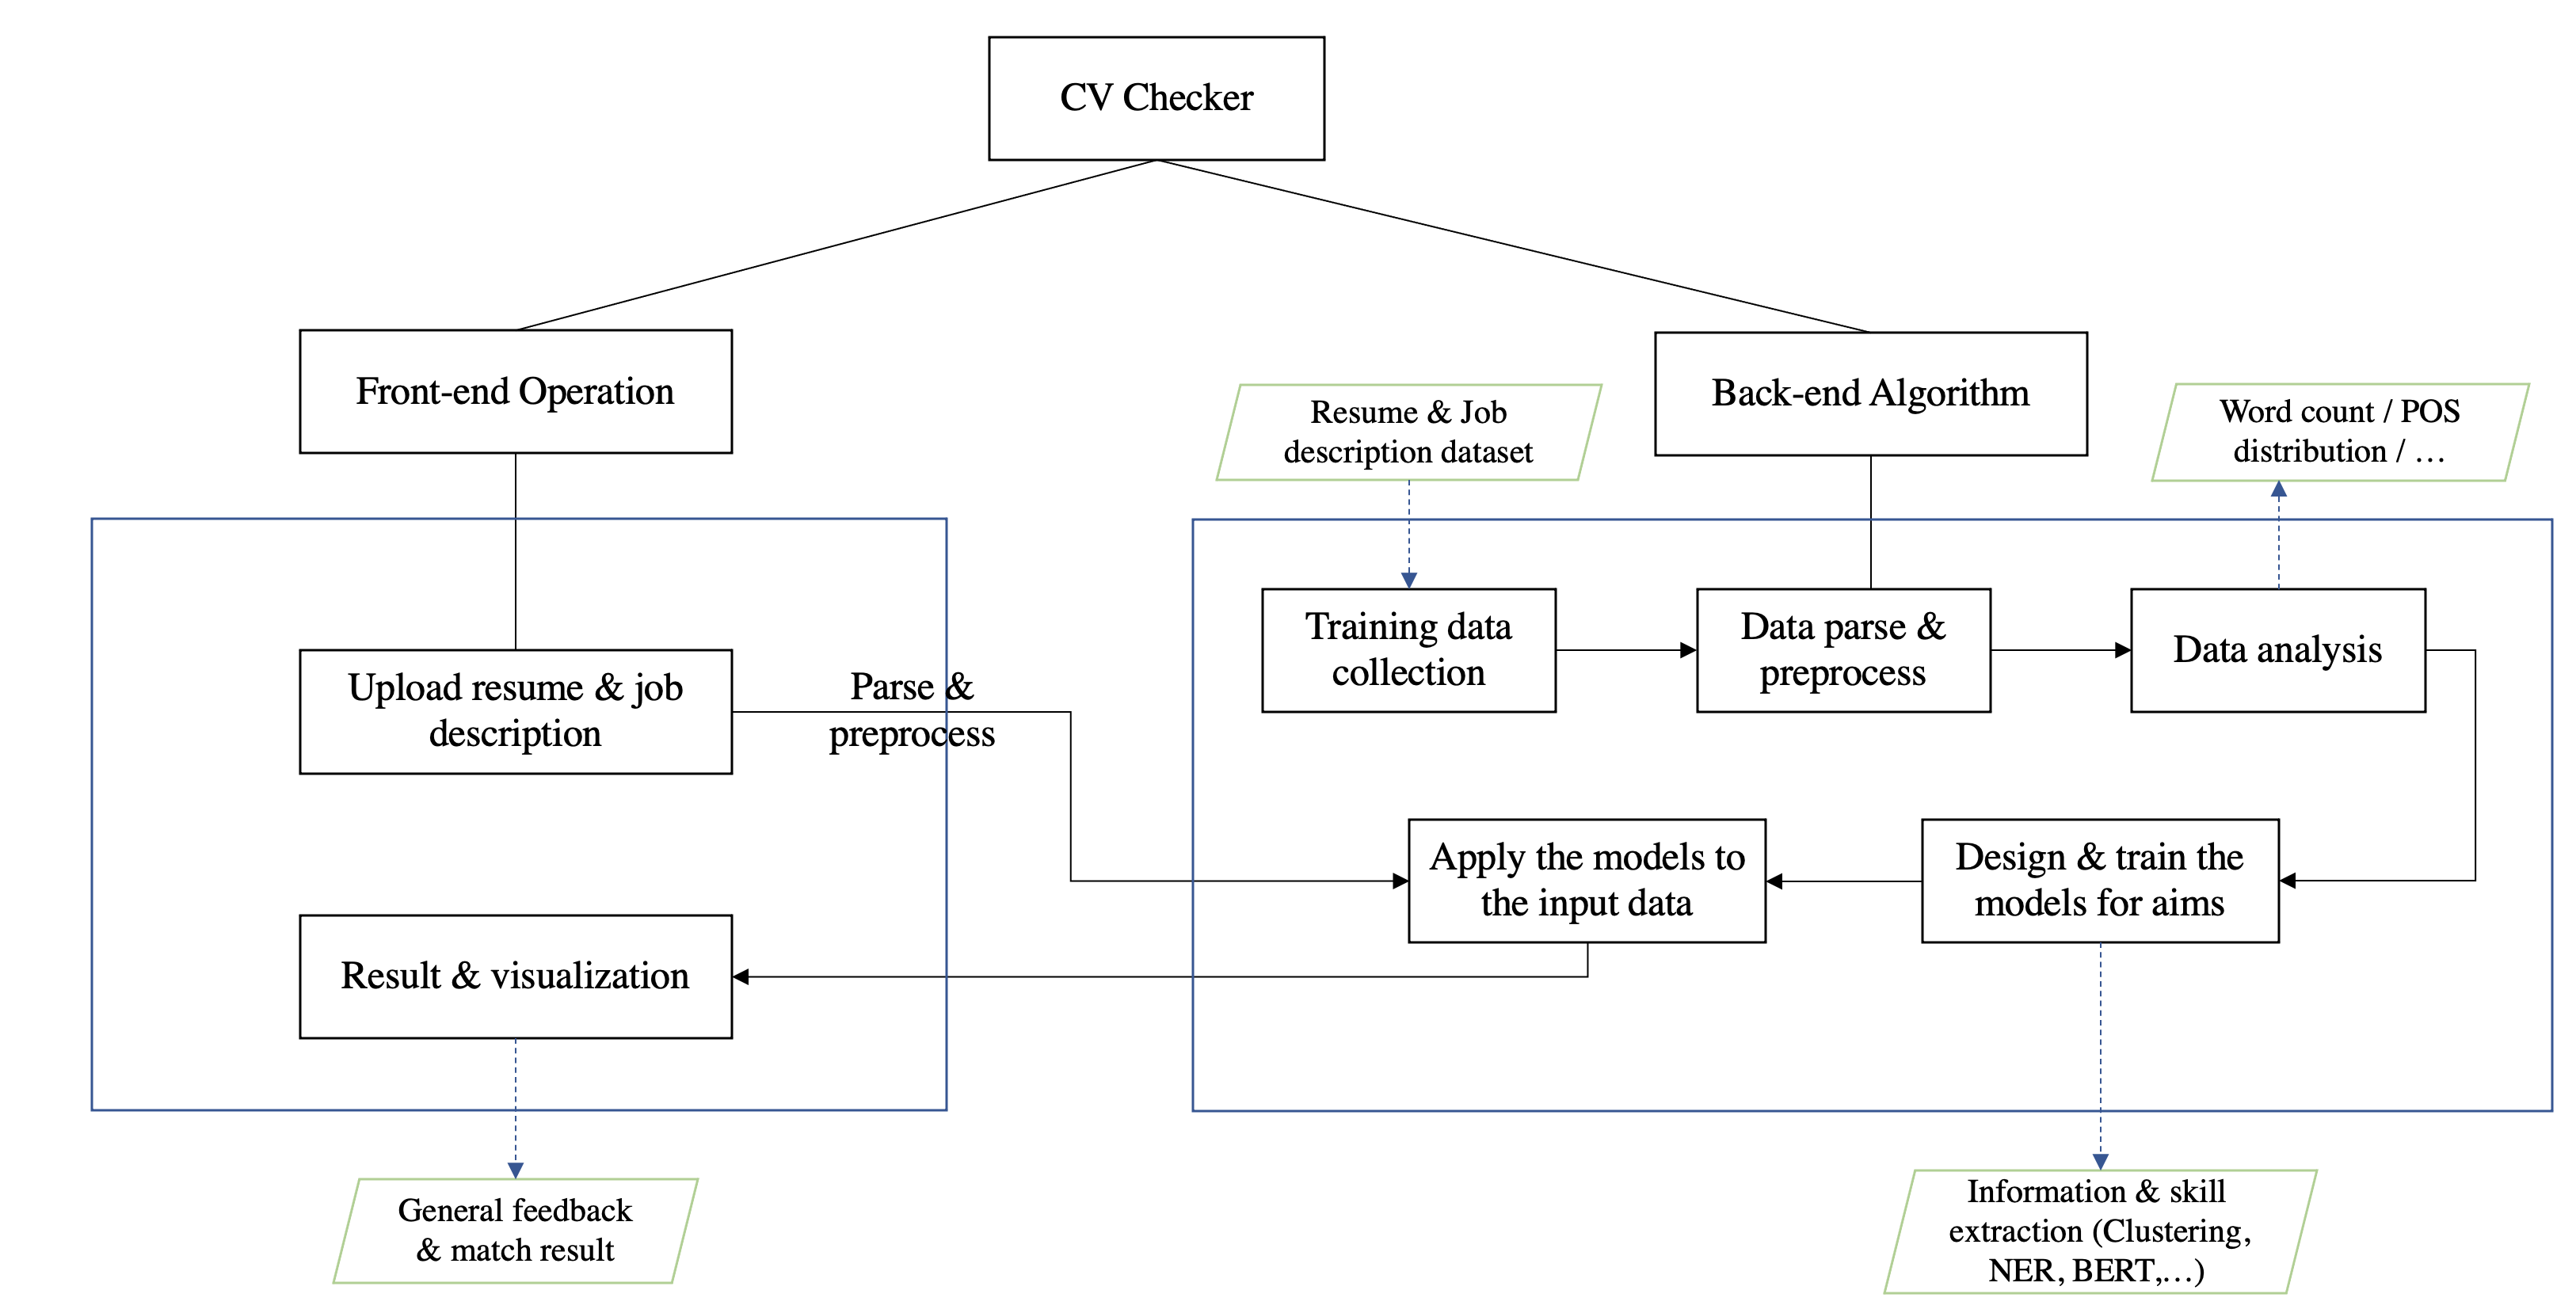
\includegraphics[width=1.2\textwidth]{images/overall_design.png}
    \caption{Overall Design}
    \label{fig:14}
\end{figure}




\section{Unified Modeling Language (UML)}

The Unified Modeling Language (UML) is a standard modeling language aiming on visualizing the design components of a software system \cite{siau2001unified}. UML includes structure diagrams and behaviour diagrams two basic types of diagrams , where structure diagrams are used to show the architecture of the system and behaviour diagrams are widely used to describe the functionalities of the system. In this section, two behaviour diagrams of this project, the sequence diagram and use case diagram, will be illustrated to represent the dynamic behaviour and functionality.

Sequence diagram depicts interactions between objects, focusing on lifelines and the message exchange between the processes. Since the interactions between the front-end and back-end in this project simply consist of uploading the resume file and the job description text data, and returning the feedback and matching result, the sequence diagram for this CV-checking website should be uncomplicated as shown in Figure \ref{fig:19}.


 \begin{figure}[H]
    \centering
    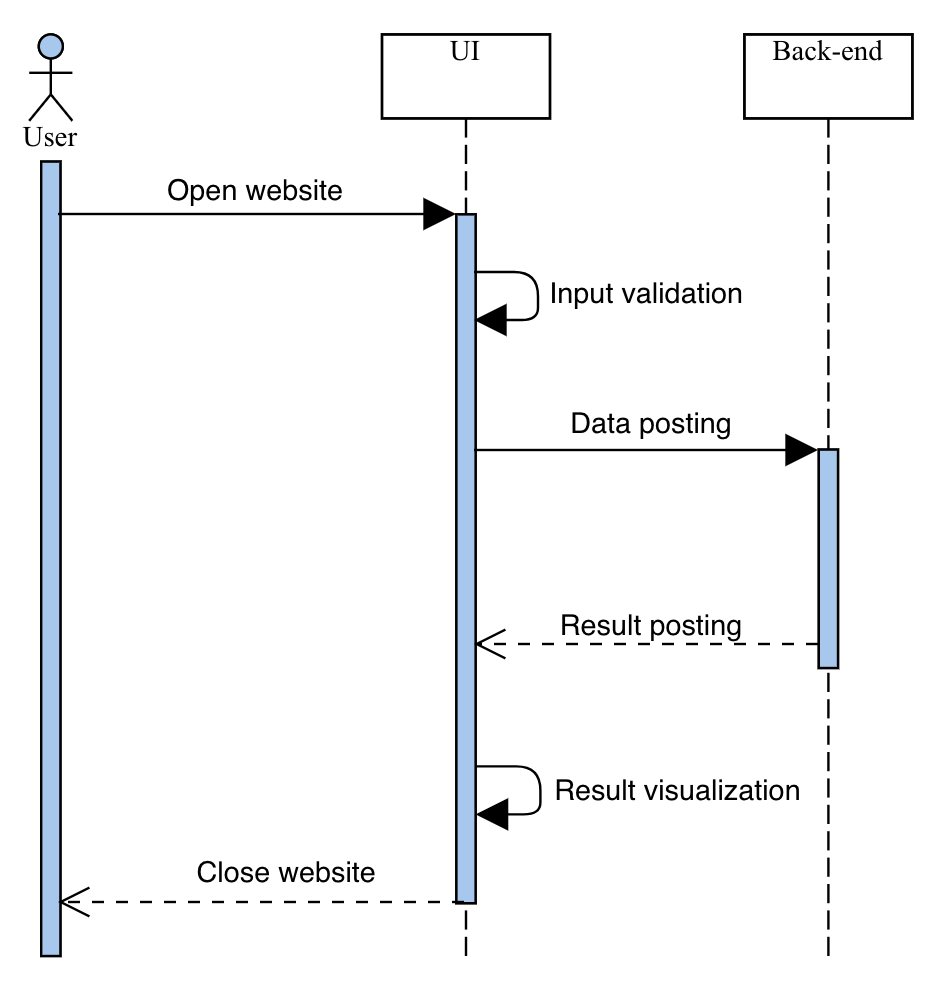
\includegraphics[width=0.6\textwidth]{images/sequence_diagram.png}
    \caption{Sequence Diagram}
    \label{fig:19}
\end{figure}

Use case diagram is also a behaviour diagram, which shows the interaction details between the actors and the system. Users and trained back-end models are regarded as the actors for our system, and the interactions are illustrated in the following Figure \ref{fig:20}.


 \begin{figure}[H]
    \centering
    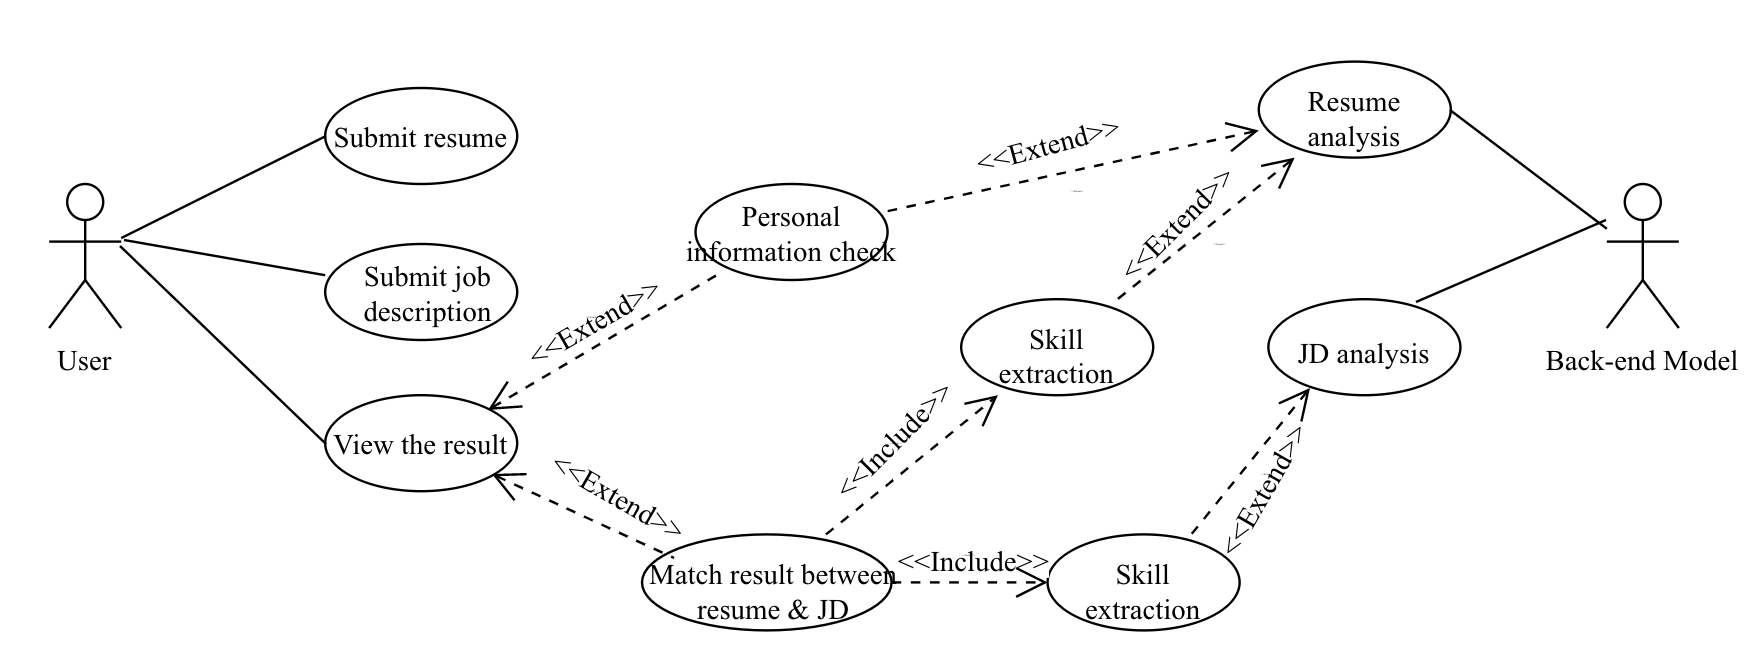
\includegraphics[width=0.9\textwidth]{images/usecase_diagram.png}
    \caption{Use Case Diagram}
    \label{fig:20}
\end{figure}


\section{User Interface}

User Interface (UI) is not set as a key objective of this project, but it still is an essential part of web development. The UI design for this project should consider the following requirements:

\begin{enumerate}
    \item The interface should be simple and straightforward.
    
    \item The website should allow users to choose a resume file and submit it. 
    
    \item The website should allow users to enter and submit the job description text.
    
    \item There should be some instructions for users to understand the usage of this application. For instance, it should be clarified which kinds of file formats could be submitted.
\end{enumerate}


 \begin{figure}[H]
    \centering
    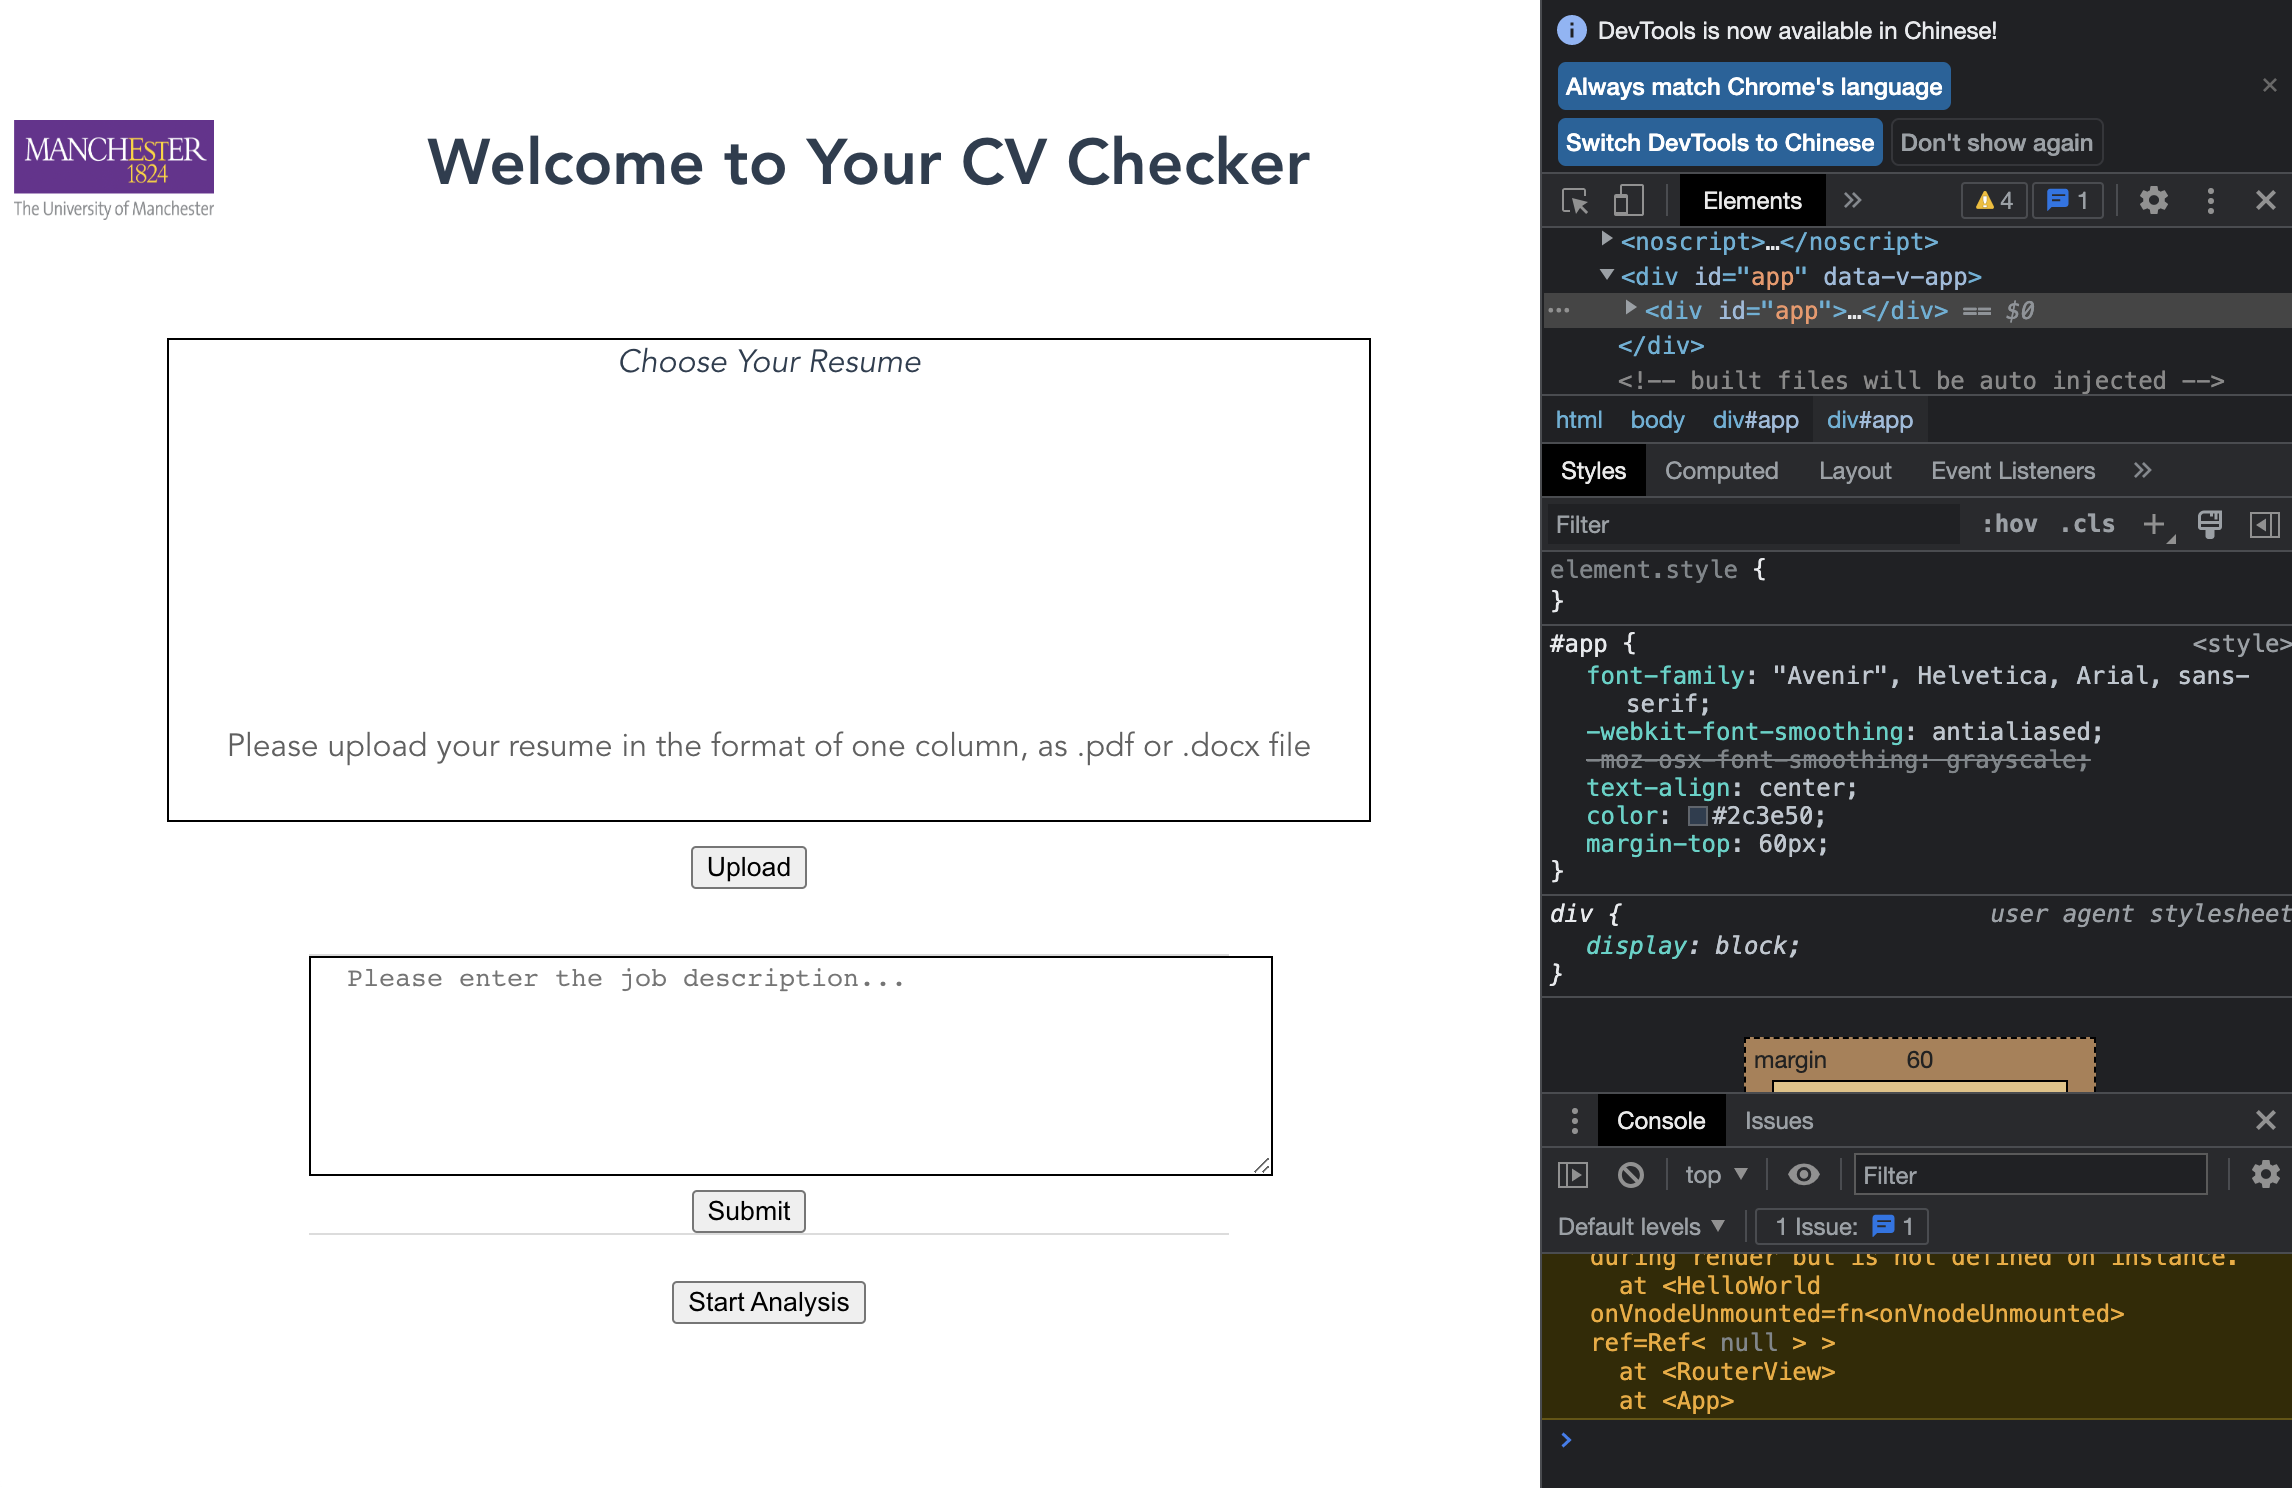
\includegraphics[width=1.2\textwidth]{images/ui.png}
    \caption{User Interface}
    \label{fig:35}
\end{figure}

Based on the design ideas, the above Figure \ref{fig:35} shows the simple user interface of the main page with the console. The top rectangle is for resume choosing and uploading, while the user can write the target job description in the bottom rectangle and submit the text. When submitting and uploading successfully, alerts would be returned on the screen. Then, the user can get the result page by pressing the 'Start Analysis' button.


\section{Data Preparation}

As illustrated in the previous section \ref{overall_design}, the resume and job description dataset should be collected for the back-end models training to implement the key information and skill extraction tasks from the input resume and job description text. This section will introduce the data preparation of the project in two parts; one is data collection, followed by the preprocessing steps for the training data in detail.

\subsection{Data Collection}
\label{sec:data}

To obtain the training data, the following requirements should be taken into consideration:

\begin{enumerate}
    \item Both resume and job description dataset should be large enough to learn the features.
    \item The resume dataset should be annotated with named entities for SpaCy NER model training, containing at least person name, e-mail address, educational information and skills , which means the label should in a specific format to point the named entities and their locations (start and end) in the data.
    \item The job description dataset is expected to cover sufficient positions from different area.
\end{enumerate}

Kaggle, a platform for data science and machine learning researchers, provides plenty of open-sourced datasets, notebooks and projects. The job description dataset used in this project is acquired from Kaggle, which contains 19,000 job postings from 2004-2015 with the content of job title, company, location, job description, job requirement, et cetera. This dataset can be accessed on \href{https://www.kaggle.com/datasets/madhab/jobposts?datasetId=1150}{Kaggle}, and has been used in multiple related tasks for job description analysis.

The resume dataset with named entities annotations is collected from an open-sourced similar project, which can be accessed on \href{https://github.com/OmkarPathak/pyresparser}{Github}. This dataset consists of 700 labeled resumes, where personal profile named entities like name, email, mobile numbers, and the entities of other information such as skills, experience, and college name are all located and annotated for NER model training.

Additionally, there is another published dataset containing multiple real-word resumes with both .pdf and .doc file format, which is available on \href{https://github.com/Msq-9/Extraction-of-Skills}{Github}. These resumes can be utilized to test our CV-checking application as the user input.

\subsection{Data Preprocessing}

Data preprocessing is a significant and essential step before applying the data to machine learning algorithms. Especially for text data, there are many structural variations of terms in the natural language and the structure of text data could be complex and inconstant \cite{kannan2014preprocessing}, which makes the preprocessing phase necessary for the tasks involving text data. The primary aims of data preprocessing is to reduce the noises, preserve the features of the text, and obtain clean and normalized data. To achieve the above goal of preprocessing, the graphical design of preprocessing pipeline is as follows in Figure \ref{fig:15}.

 \begin{figure}[H]
    \centering
    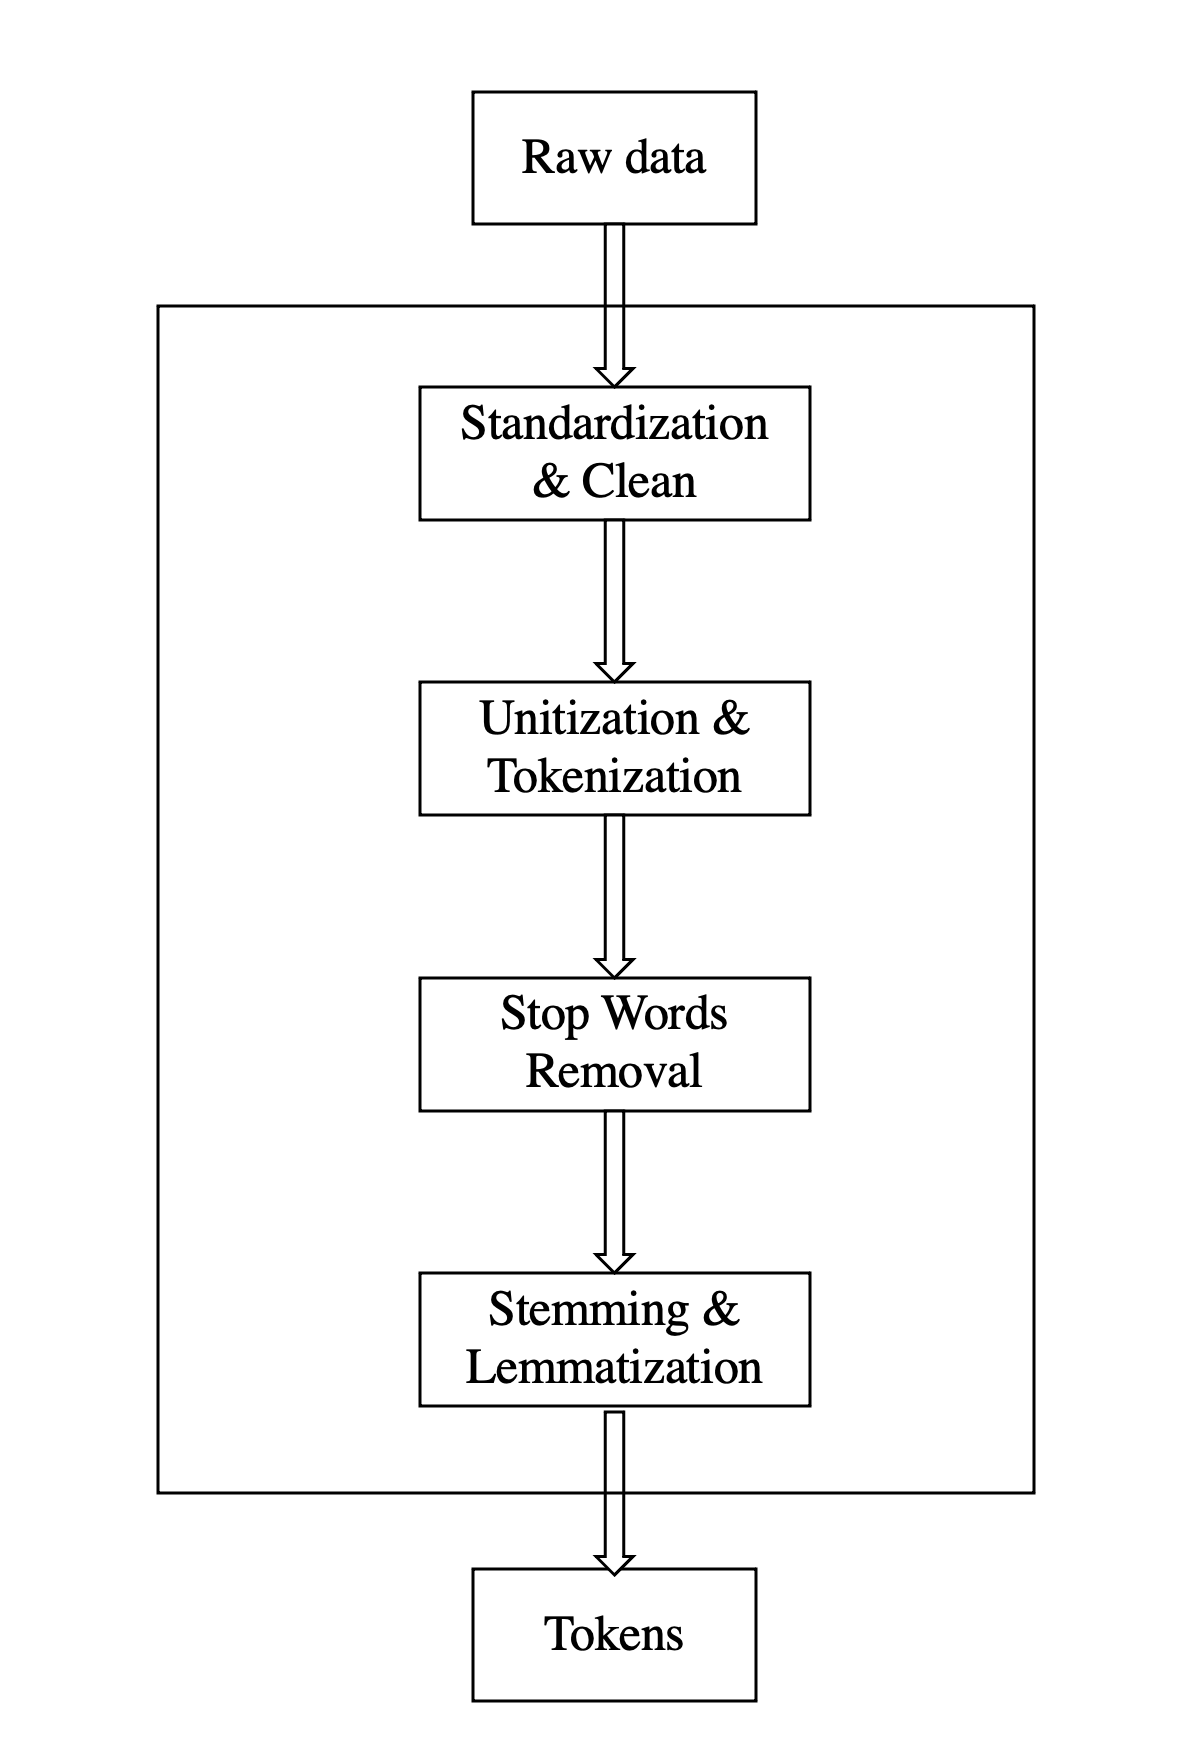
\includegraphics[width=0.45\textwidth]{images/preprocessing.png}
    \caption{Preprocessing Pipeline}
    \label{fig:15}
\end{figure}

The main steps of data preprocessing include: 1) standardizing and cleaning the data by removing punctuation, special characters and format using regular expressions, 2) unitization and tokenization to get smaller units from the document to understand the data structure, in terms of sentence tokens and word tokens, then lower case all the tokens, 3) removing the stop words such as pronouns and preposition by NLTK stop words list, 4) stemming and lemmatization, then tagging with POS. As introduced in Section \ref{method_preprocessing}, NLTK is used as the tool for the above preprocessing processes. Moreover, after preprocessing the data, visualization techniques such as word cloud and histogram will be used for data analysis to show the keywords and word distribution. The examples of the visualization result are as follows. Through manual check, the related words computed by word vectors are reasonable, which means this word2vec model performs well.

\begin{figure}[H]
    \begin{minipage}[t]{0.5\linewidth}
        \centering
        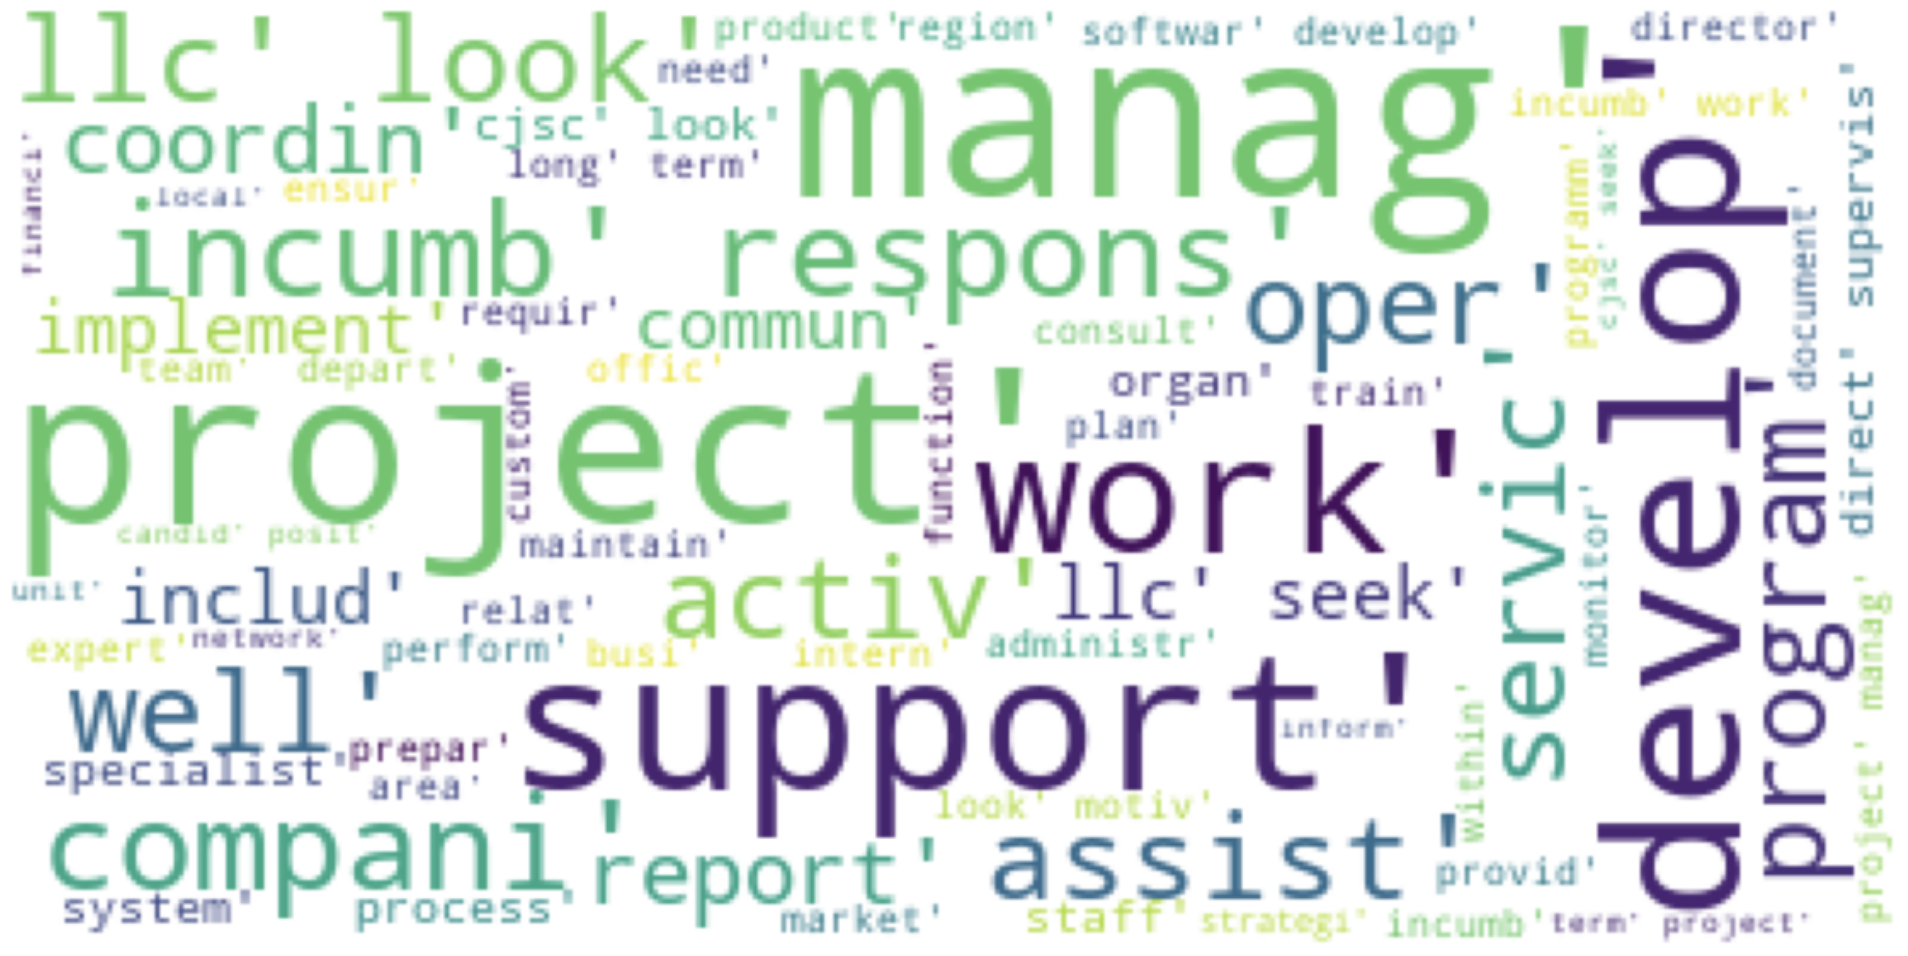
\includegraphics[scale=0.2]{images/wordcloud_exp.png}
        % \caption{Word Cloud}
        \label{fig:16}
    \end{minipage}%
    \begin{minipage}[t]{0.5\linewidth}
        \centering
        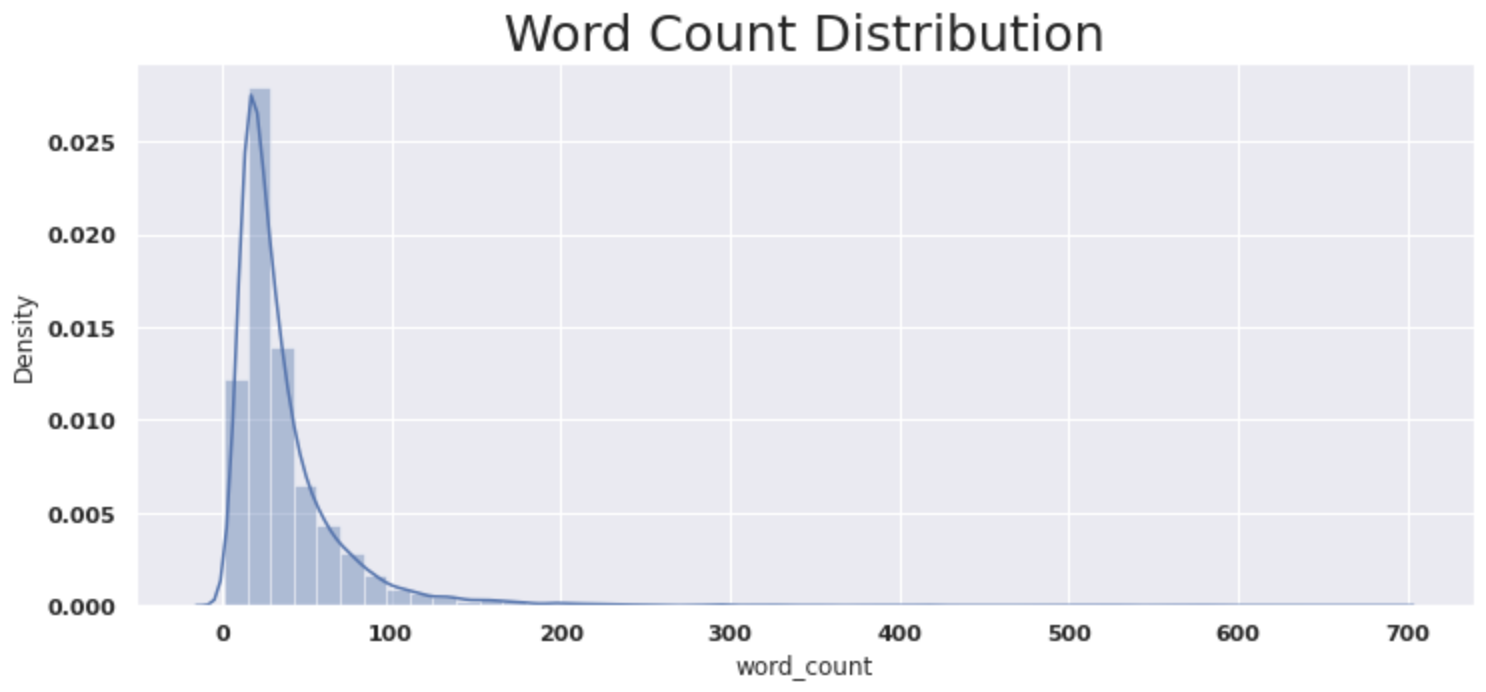
\includegraphics[scale=0.3]{images/distribution_exp.png}
        % \caption{Histogram}
        \label{fig:17}
    \end{minipage}
    \caption{Example of Visualization}
\end{figure}

By using the word vectors as the training samples, K-means algorithm could be applied to get the clusters. 

\section{Back-end Algorithms}
\label{sec:backend_design}

With the preprocessed training data, back-end algorithms are designed to recognize key information, extract skills and compute the match rate tasks like the existing CV checkers such as \href{https://www.jobscan.co/}{Jobscan}. The following specifications should be considered when designing models:

\begin{enumerate}
    \item The system should be able to understand the content of the submitted new resume and check the coverage of basic information such as person name, email address, educational detail, etc.
    
    \item The system should be able to extract the skills mentioned in the submitted resume.
    
    \item The system should be able to discover the requirements of the position from the job description by skill extraction.
    
    \item The system should enable to match the person's skills and the position requirements, and return the match rate combined with detailed result.
\end{enumerate}

 \begin{figure}[H]
    \centering
    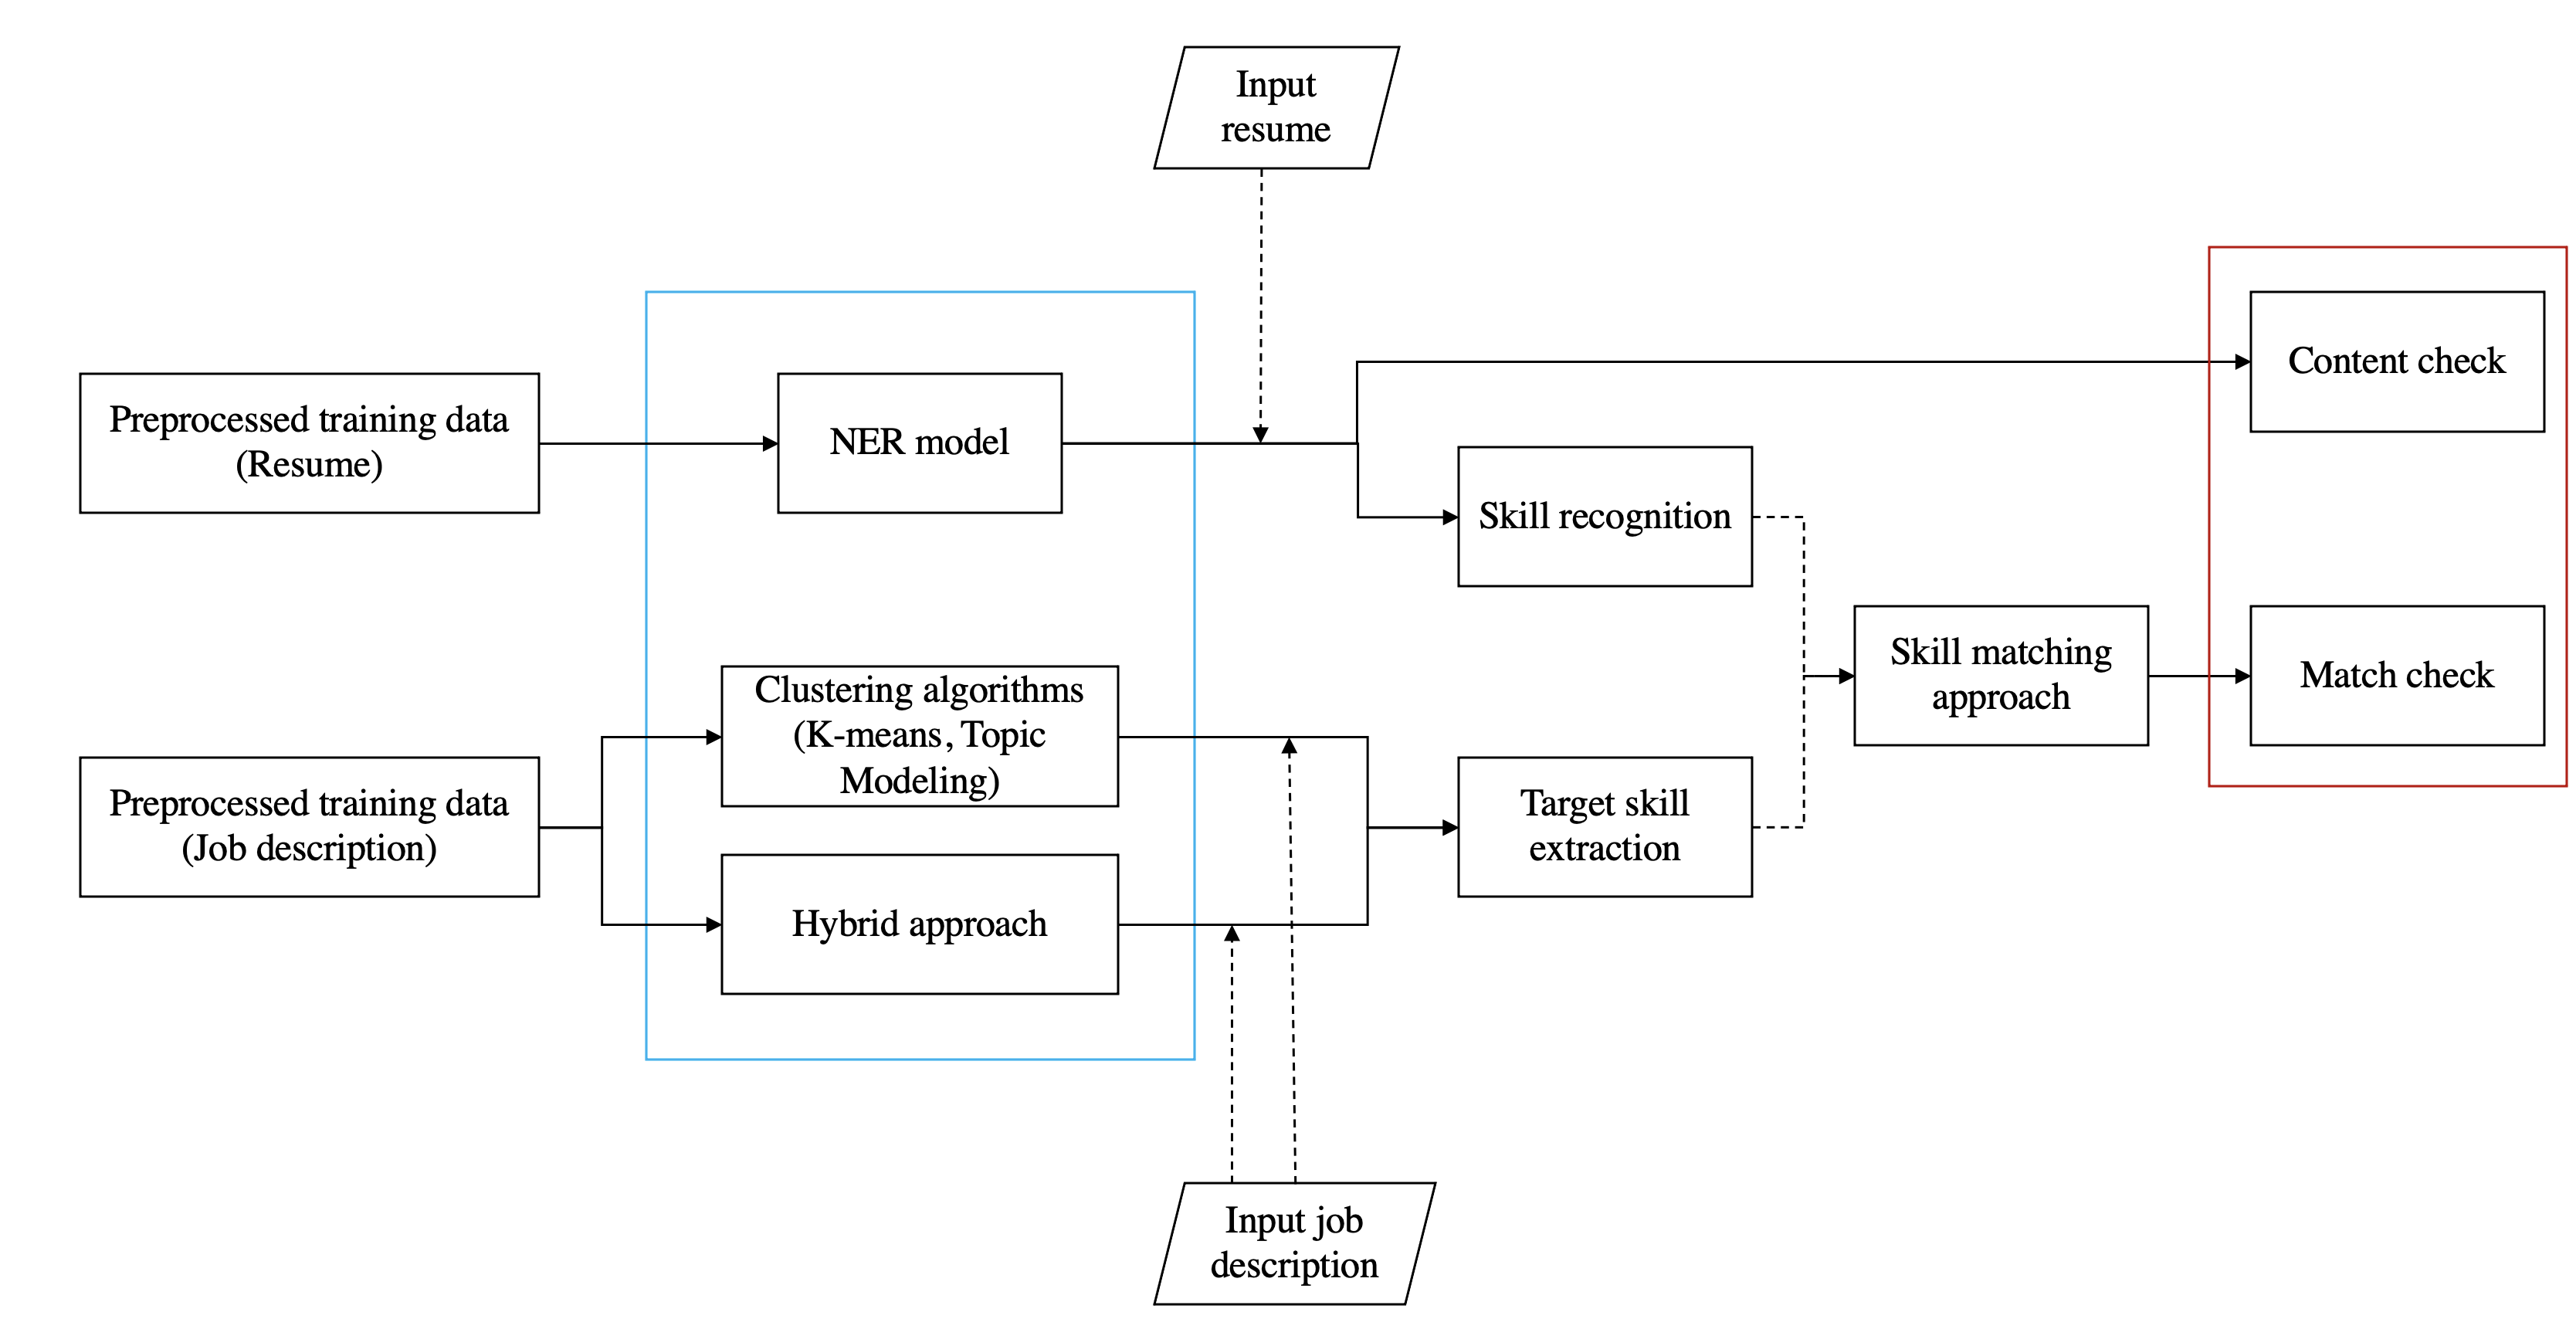
\includegraphics[width=1.2\textwidth]{images/backend_design.png}
    \caption{Back-end System Design}
    \label{fig:18}
\end{figure}

In order to fulfill the specifications, the general design of the back-end system is presented in the above diagram \ref{fig:18}. Because the inside algorithms of the existing CV checkers could not be known to the public, though the functionalities of our project refer to the existing CV checker, the implementation of the functionalities is like a black box for us. In this case, various approaches, which have been described in Chapter \ref{ch:methodology}, need to be experimented during the development to find a suitable approach for target tasks. In the diagram of the back-end design, the blue area refers to the experimented models and approaches to implement different functionalities, the dashed arrows denote applying the input data to the trained models for prediction or extraction, and the red area means the two final targets. As for the aim of the content check, preprocessed resume data is used to train an NER model, which will be applied to the input resume to check the coverage of the necessary information. Since the training dataset contains the skill annotation as well, the NER model could also be used to recognize the skills from the input resume. For the target of the match check, besides skill extraction from the input resume, the skills in the uploaded job description should also be identified. The preprocessed job description dataset should be used as the training set, and experiments on different approaches are needed for the extraction task. With the extracted skills from the input resume and job description, the skill matching approach can be used for the match check.

Chapter \ref{ch:methodology} introduced several libraries to train the models for the CV checker. NER model training for the content check is implemented by spaCy, K-means clustering training is provided by Scikit-learn, and LDA topic model can be achieved by Gensim. 

As for the hybrid approach for determining skills in the job description, the basic processes have been shown in section \ref{sec:hybrid}. After tagging the POS of tokens by NLTK, regular expression chunking techniques should be used to obtain reasonable chunks. According to \cite{ketterer}, skills usually appear in four kinds of patterns, and their regular expressions are described as follows:

\begin{enumerate}
    \item Basic Noun Phrase: including singular and plural noun, proper noun, noun with a determinate, and noun with adjectives. The regular expression can be written as $\{<DT>?<JJ>*<NN|NNS|NNP>+\}$, where $"?"$ means optional included, $"*"$ refers to any number of tags included and $+$ means including one or more. $DT$ is the POS tag for determiner, $JJ$ means adjective, $NN$, $NNS$, $NNP$ are singular noun, plural noun and proper noun separately.
    
    \item Variation of Noun Phrase: containing an optional preposition or conjunction, followed by nouns or adjectives and ending with a singular noun or plural noun. Its regular expression is $\{<IN>?<JJ|NN>*<NNS|NN>\}$, where $IN$ is the POS tag for preposition.
    
    \item Verb Phrase: including all kinds of verbs followed by a singular noun or plural noun. The regular expression is $<VBG|VBZ|VBP|VBD|VB|VBN><NNS|NN>*$
    
    \item Nouns splitted by comma: this situation is considered because some of the job descriptions might list the expected requirements (skills) separated by comma. The regular expression could be $<NN|NNS>*<,><NN|NNS>*<,><NN|NNS>*$
    
\end{enumerate}

After defining the regular expressions of the patterns, NLTK RegexChunkParser can find the chunks in the text by using those regular expressions as the rules. Manually labeling the chunks, the training dataset is prepared. The subsequent neural network with BERT layer is built based on Keras, an API for high-level neural networks running on top of the TensorFlow machine learning platform \cite{keras}. The architecture of the deep learning neural network with BERT layer is shown in the following Figure \ref{fig:12}.

 \begin{figure}[H]
    \centering
    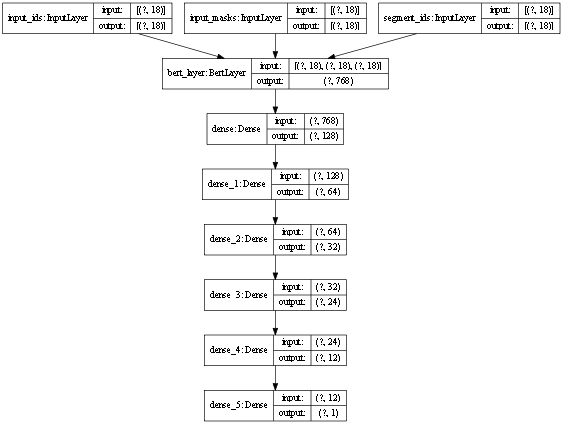
\includegraphics[width=0.9\textwidth]{images/withBERT.png}
    \caption{Architecture of Neural Network \cite{ketterer2}}
    \label{fig:12}
\end{figure}

With the extracted skills from the resume and the job description, the match rate can be obtained by calculating the cosine similarity from the text.
% skill matching implementation

% \section{Visualization Result}

